\documentclass[12pt,a4paper]{article}
\usepackage[utf8]{inputenc}
\usepackage[spanish]{babel}
\usepackage{amsmath}
\usepackage{amsfonts}
\usepackage{amssymb}
\usepackage{graphicx}
\usepackage[left=2cm,right=2cm,top=2cm,bottom=2cm]{geometry}
\author{Enciso Guerrero Benjamin Salvador\\
Carlos Enrrique Moran Garabito\\
Cinematica De Robots }
\title{Métodos geométricos, algebraico y desacopio cinemático.}
\begin{document}
\maketitle

\includegraphics[scale=1.8]{upzmgg.jpg} 
\newpage
Método geométrico.
\\\\
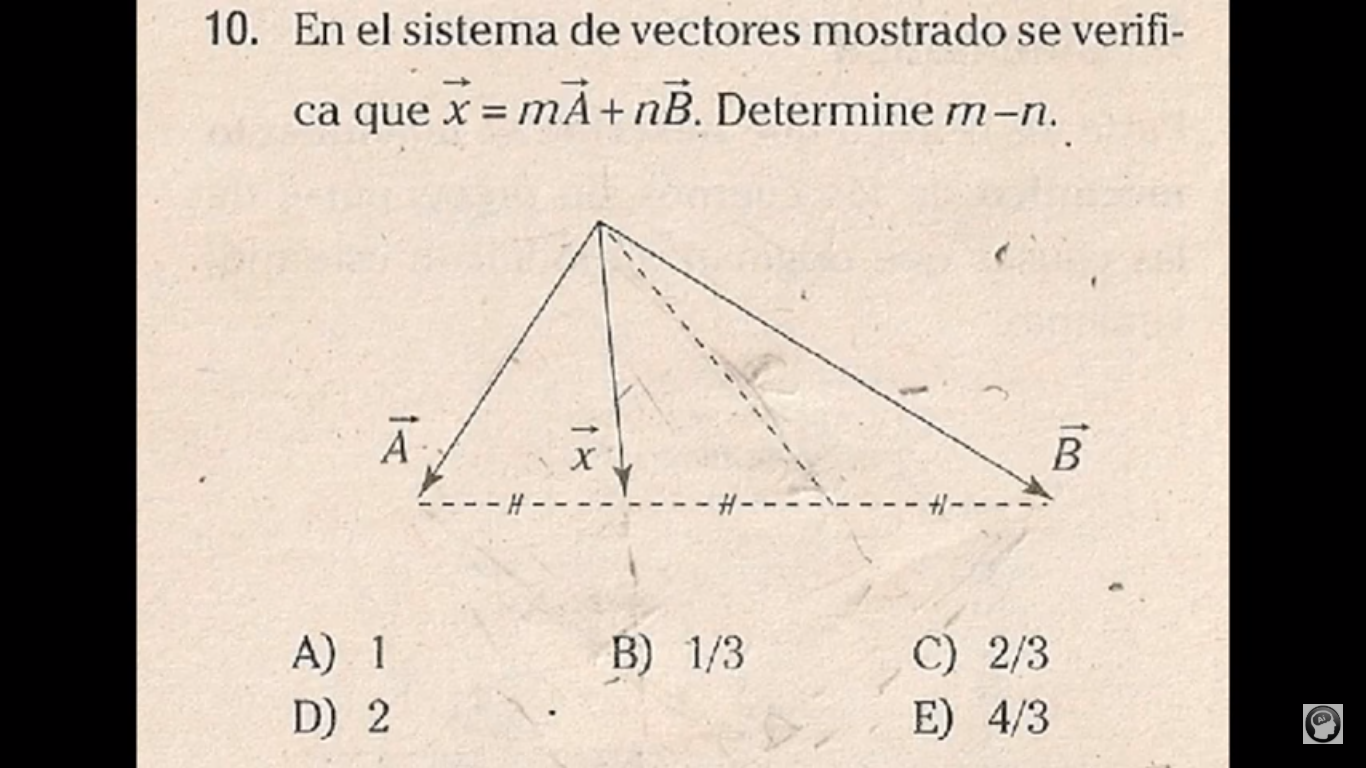
\includegraphics[scale=0.47]{imagen1.png} 
\\\\
En principio tenemos que recordar que si tenemos un vector de dos barras o dos trazos como el de la siguiente imagen:
\\\\
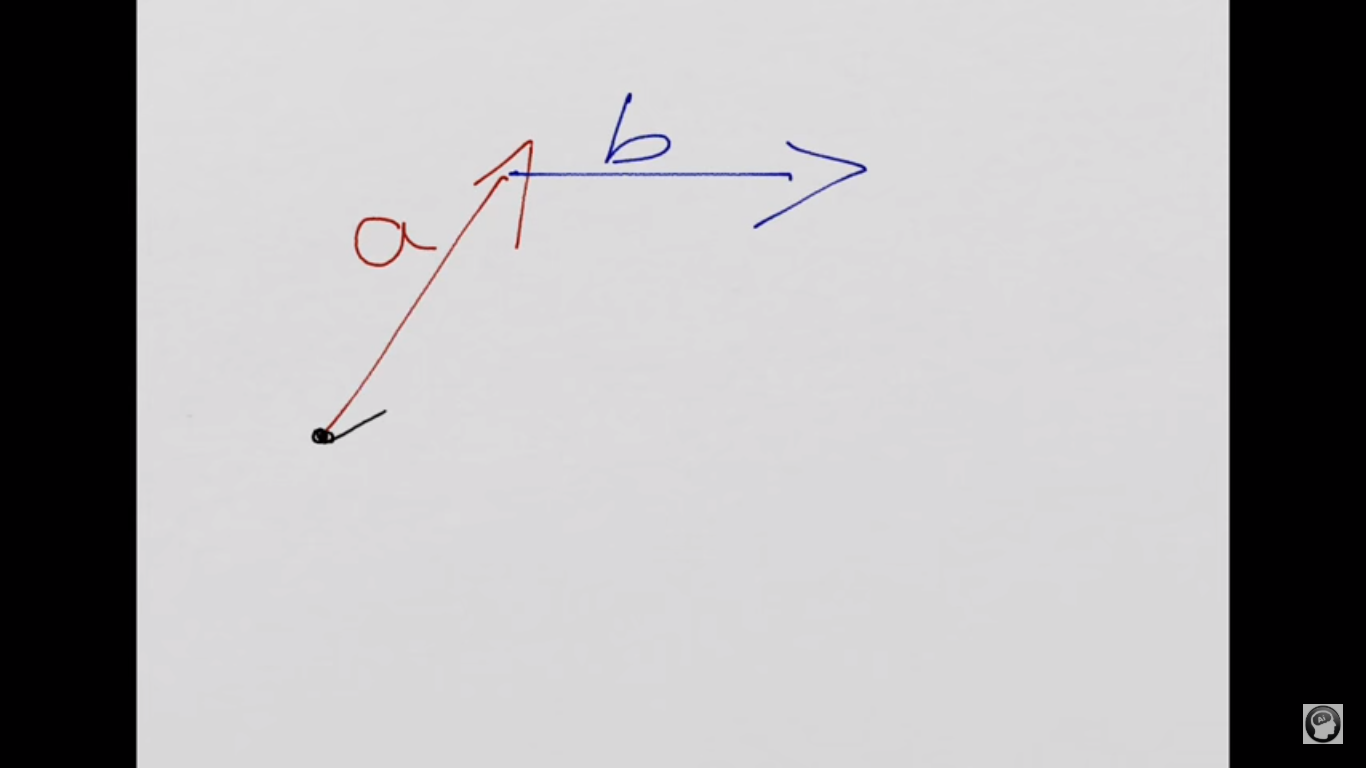
\includegraphics[scale=0.47]{imagen2.png} 
\\\\
\newpage
La resultante va a ser de a+b.
\\\\
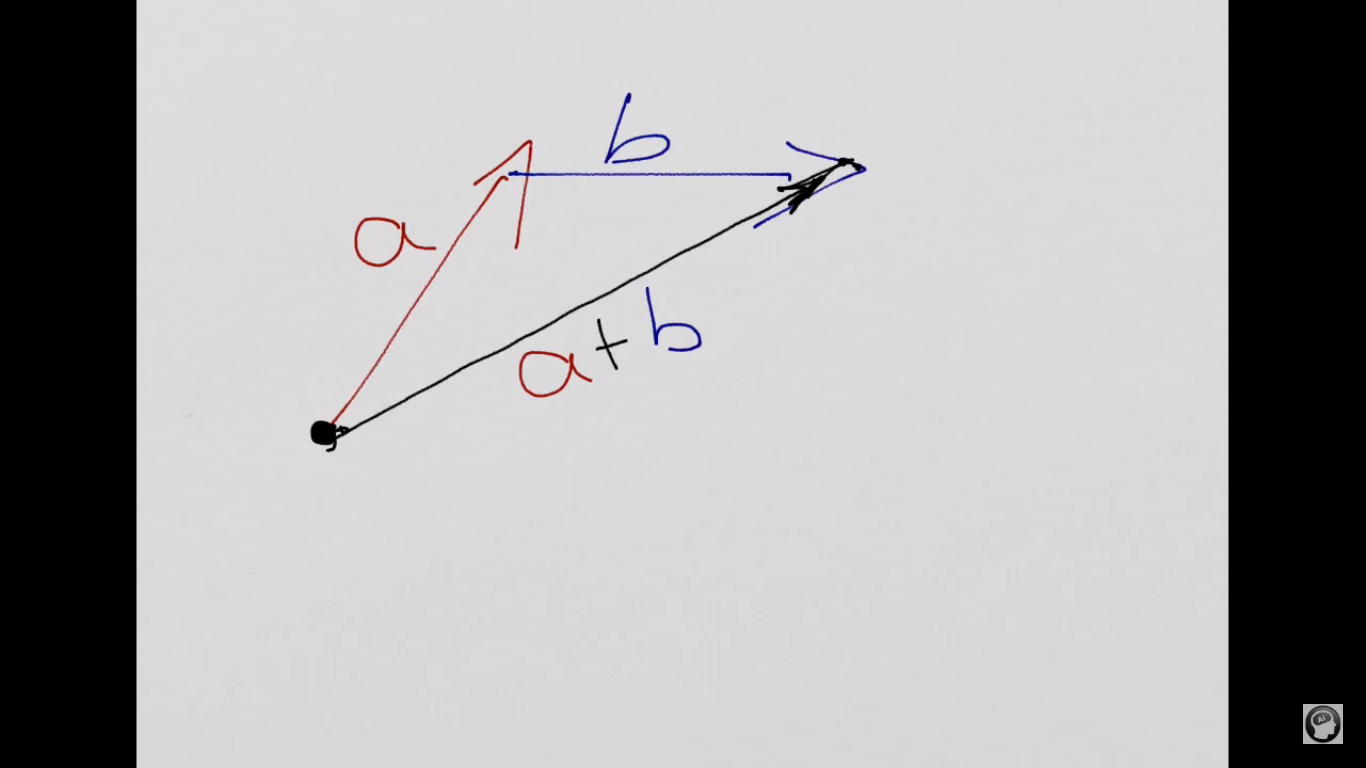
\includegraphics[scale=0.47]{imagen3.png} 
\\\\
Recordando esto, así es como se determina la resultante de dos vectores geométricamente.
\\\\
\title{Método algebraico}
\\\\
El método de balanceo algebraico se basa en el planteamiento de un sistema de ecuaciones en la cual los coeficientes estequiométricos participan como incógnitas, procediendo luego despejar estas incógnitas.
\\\\
Es posible sin embargo que muchas veces queden planteados sistemas de ecuaciones con más incógnitas que ecuaciones, en esos casos la solución se halla igualando a uno de cualquiera de los coeficientes a 1 y luego despejando el resto en relación a él. 
\\\\
Finalmente se multiplican todos los coeficientes por un número de modo tal de encontrar la menor relación posible entre coeficientes enteros.
\\\\\\\\
\title{
Desacopio cinemático
}
\\\\
Concepto:
\\
Habitualmente los tres últimos ejes del robot se cortan en un punto.
\\
La finalidad de estos es lograr la orientación de la herramienta, aunque como consecuencia de su movimiento tengan un efecto ligero sobre la posición.
\\
Con la primera condición se puede simplificar enormemente el problema cinemático para 6 gdl, dado que la obtención de este punto de intersección es una operación sencilla.
\\
Este punto dependerá sólo de los 3 primeros gdl, por lo que su obtención es asequible.

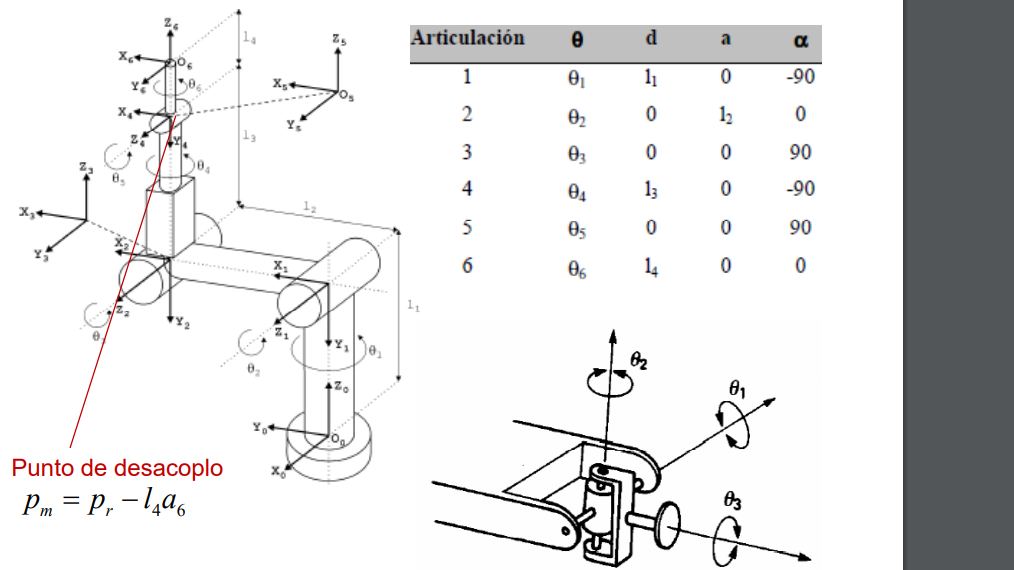
\includegraphics[scale=0.6]{imagen4.png} 
\\\\
Resolviendo:
\\\\\\
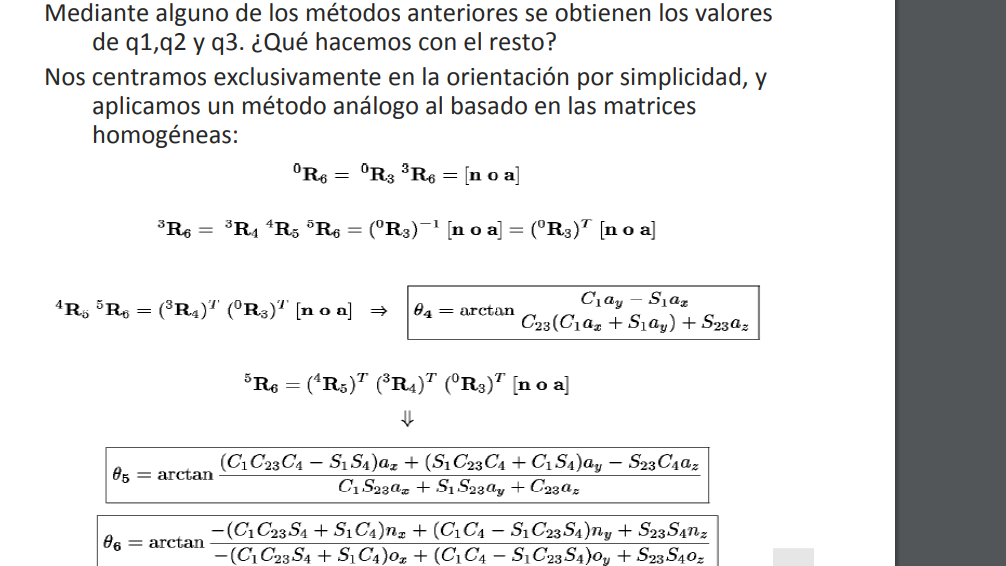
\includegraphics[scale=0.6]{imagen5.png} 
\end{document}